\documentclass[
    article,
	% -- opções da classe memoir --
	12pt,				% tamanho da fonte
	openright,			% capítulos começam em pág ímpar (insere página vazia caso preciso)
	oneside,			% para impressão em verso e anverso. Oposto a oneside
	a4paper,			% tamanho do papel. 
	% -- opções da classe abntex2 --
	%chapter=TITLE,		% títulos de capítulos convertidos em letras maiúsculas
	section=TITLE,		% títulos de seções convertidos em letras maiúsculas
	%subsection=TITLE,	% títulos de subseções convertidos em letras maiúsculas
	%subsubsection=TITLE,% títulos de subsubseções convertidos em letras maiúsculas
	% -- opções do pacote babel --
	%english,			% idioma adicional para hifenização
	%french,				% idioma adicional para hifenização
	%spanish,			% idioma adicional para hifenização
	brazil				% o último idioma é o principal do documento
	]{abntex2}

\usepackage{ifthen,ifpdf}

\ifpdf
  \pdfpagewidth=\paperwidth
  \pdfpageheight=\paperheight
\fi

% --- 
% CONFIGURAÇÕES DE PACOTES
% --- 
% ---
% Pacotes básicos 
% ---
\usepackage{lmodern}			% Usa a fonte Latin Modern			
\usepackage[T1]{fontenc}		% Selecao de codigos de fonte.
\usepackage[utf8]{inputenc}		% Codificacao do documento (conversão automática dos acentos)
\usepackage{lastpage}			% Usado pela Ficha catalográfica
\usepackage{indentfirst}		% Indenta o primeiro parágrafo de cada seção.
\usepackage{color}				% Controle das cores
\usepackage{graphicx}			% Inclusão de gráficos
\usepackage{microtype} 			% para melhorias de justificação
\usepackage{ufc-abntex2}
\usepackage{enumitem}
\usepackage{amsmath}
\usepackage{booktabs}
\usepackage{multirow}
\usepackage{titlesec}

%formatação do Sumário
\usepackage{etoolbox}                               
% Usado para alterar a fonte da Section no Sumário
\usepackage[nogroupskip,nonumberlist,acronym]{glossaries}                %
% ---
		
% ---
% Pacotes adicionais, usados apenas no âmbito do Modelo Canônico do abnteX2
% ---
\usepackage{lipsum}				% para geração de dummy text
% ---

% ---
% Pacotes de citações
% ---
%\usepackage[brazilian,hyperpageref]{backref}	 % Paginas com as citações na bibl
%\usepackage[alf]{abntex2cite}	% Citações padrão ABNT

%Com et al nas referências
%\usepackage[alf, abnt-emphasize=bf, bibjustif, recuo=0cm, abnt-etal-cite=3, abnt-etal-text=it, abnt-etal-list=3]{abntex2cite} 

%Sem et al nas referências
\usepackage[alf, abnt-emphasize=bf, bibjustif, recuo=0cm, abnt-etal-cite=3, abnt-etal-text=it, abnt-etal-list=0]{abntex2cite} 

% Ambiente para alineas e e subalineas (incisos) com ponto
\newlist{alineascomponto}{itemize}{2}
\setlist[alineascomponto,1]{label={$\bullet$},topsep=0pt,itemsep=0pt,leftmargin=\parindent+\labelwidth-\labelsep}%
\setlist[alineascomponto,2]{label={--},topsep=0pt,itemsep=0pt,leftmargin=*}
\newlist{subalineascomponto}{enumerate}{1}
\setlist[subalineascomponto,1]{label={$\circ$},topsep=0pt,itemsep=0pt,leftmargin=*}%
% ---

% Ambiente para alineas e e subalineas (incisos) com numeros
\newlist{alineascomnumero}{enumerate}{2}
\setlist[alineascomnumero,1]{label={$\arabic*$.},topsep=0pt,itemsep=0pt,leftmargin=\parindent+\labelwidth-\labelsep}%
\setlist[alineascomnumero,2]{label={--},topsep=0pt,itemsep=0pt,leftmargin=*}
\newlist{subalineascomnumero}{enumerate}{1}
\setlist[subalineascomnumero,1]{label={$\arabic*$.},topsep=0pt,itemsep=0pt,leftmargin=*}%
% ---

% ---
% Configurações do pacote backref
% Usado sem a opção hyperpageref de backref
%\renewcommand{\backrefpagesname}{Citado na(s) página(s):~}
% Texto padrão antes do número das páginas
%\renewcommand{\backref}{}
% Define os textos da citação
%\renewcommand*{\backrefalt}[4]{
%	\ifcase #1 %
%		Nenhuma citação no texto.%
%	\or
%		Citado na página #2.%
%	\else
%		Citado #1 vezes nas páginas #2.%
%	\fi}%
% ---

% ---
% Configurações de aparência do PDF final

% alterando o aspecto da cor azul
\definecolor{blue}{RGB}{41,5,195}

% informações do PDF
\makeatletter
\hypersetup{
     	%pagebackref=true,
		pdftitle={\@title}, 
		pdfauthor={\@author},
    	pdfsubject={\imprimirpreambulo},
	    pdfcreator={LaTeX with abnTeX2},
		pdfkeywords={abnt}{latex}{abntex}{abntex2}{trabalho acadêmico}, 
		colorlinks=true,       		% false: boxed links; true: colored links
    	linkcolor=blue,          	% color of internal links
    	citecolor=blue,        		% color of links to bibliography
    	filecolor=magenta,      		% color of file links
		urlcolor=blue,
		bookmarksdepth=4
}
\makeatother
% --- 

\makeatletter
\def\@biblabel#1{}
\renewenvironment{thebibliography}[1]
     {\section*{\refname}%
      \@mkboth{\MakeUppercase\refname}{\MakeUppercase\refname}%
      \list{\@biblabel{\@arabic\c@enumiv}}%
           {\settowidth\labelwidth{\@biblabel{#1}}%
            \leftmargin\labelwidth
            %\advance\leftmargin\labelsep
            \@openbib@code
            \usecounter{enumiv}%
            \let\p@enumiv\@empty
            \renewcommand\theenumiv{\@arabic\c@enumiv}}%
      \sloppy
      \clubpenalty4000
      \@clubpenalty \clubpenalty
      \widowpenalty4000%
      \sfcode`\.\@m}
     {\def\@noitemerr
       {\@latex@warning{Empty `thebibliography' environment}}%
      \endlist}
\makeatother

% --- 
% Espaçamentos entre linhas e parágrafos 
% --- 

% O tamanho do parágrafo é dado por:
\setlength{\parindent}{1.3cm}

% Controle do espaçamento entre um parágrafo e outro:
\setlength{\parskip}{0.2cm}  % tente também \onelineskip

% ---
% compila o indice
% ---
\makeindex
% ---


% Define as margens do documento
\setlrmarginsandblock{3cm}{2cm}{*} % externa / interna
\setulmarginsandblock{3cm}{2cm}{*} % superior / inferior


\usepackage{hyperref}% http://ctan.org/pkg/hyperref
\hypersetup{%
  colorlinks = false,
  linkcolor  = black
}

% Informações de dados para CAPA e FOLHA DE ROSTO
\titulo{TÍTULO TÍTULO TÍTULO TÍTULO  TÍTULO TÍTULO TÍTULO TÍTULO TÍTULO TÍTULO TÍTULO TÍTULO TÍTULO TÍTULO }
\autor{Nome Autor}
\local{Quixadá}
\data{Abril, 2016}
\orientador{Nome Orientador}
\coorientador{Nome Coorientador}

% Escolher curso: Redes de Computadores (rc), Eng.Software (es), Ciências da Computação (cc) ou Sist.Informação (si)
%\instituicao{%
Universidade Federal do Ceará \par
Campus Quixadá \par
Curso de Redes de Computadores
}
\tipotrabalho{Trabalho de Conclusão de Curso (Monografia)}
\preambulo{Monografia apresentada ao Curso de Redes de Computadores do Campus Quixadá da Universidade Federal do Ceará, como requisito parcial para obtenção do Título de Tecnólogo em Redes de Computadores.}

%\instituicao{%
Universidade Federal do Ceará \par
Campus Quixadá \par
Curso de Sistemas de Informação
}
\tipotrabalho{Trabalho de Conclusão de Curso (Monografia)}
\preambulo{Monografia apresentada ao Curso de Sistemas de Informação do Campus Quixadá da Universidade Federal do Ceará, como requisito parcial para obtenção do Título de Bacharel em Sistemas de Informação.}

\instituicao{
Universidade Federal do Ceará \par
Campus de Quixadá \par
Curso de Engenharia de Software
}

\ies{Universidade Federal do Ceará}
\campus{Campus de Quixadá}
\curso{Curso de Engenharia de Software}

\tipotrabalho{Trabalho de Conclusão de Curso (Monografia)}
\preambulo{Monografia apresentada ao Curso de Engenharia de Software do Campus Quixadá da Universidade Federal do Ceará, como requisito parcial para obtenção do Título de Bacharel em Engenharia de Software.}

%\instituicao{%
Universidade Federal do Ceará \par
Campus Quixadá \par
Curso de Ciências da Computação
}
\tipotrabalho{Trabalho de Conclusão de Curso (Monografia)}
\preambulo{Monografia apresentada ao Curso de Ciências da Computação do Campus Quixadá da Universidade Federal do Ceará, como requisito parcial para obtenção do Título de Bacharel em Ciências da Computação.}
 

%%criar um novo estilo de cabeçalhos e rodapés
\makepagestyle{header_style}
  %%cabeçalhos
  \makeoddhead{header_style} %%pagina ímpar ou com oneside
     {}
     {}
     {\thepage} 


\begin{document}
\frenchspacing 

%Formatação de título de seções
\titleformat{\section}
{\normalfont\normalsize\bfseries}{\thesection}{1em}{}
\titleformat{\subsection}
{\normalfont\normalsize\bfseries}{\thesubsection}{1em}{}
\titleformat{\subsubsection}
{\normalfont\normalsize\bfseries}{\thesubsubsection}{1em}{}

\renewcommand{\cftsectionfont}{\normalfont\normalsize}   
\renewcommand{\cftsubsectionfont}{\normalfont\normalsiz} 
\renewcommand{\cftsubsubsectionfont}{\normalfont\normalsize}  

% ----------------------------------------------------------
% ELEMENTOS PRÉ-TEXTUAIS
% ----------------------------------------------------------
% \pretextual
% Capa
\imprimircapa

%----------- Apenas TCC 2
% Folha de rosto (* indica que haverá a ficha bibliográfica)
%\imprimirfolhaderosto

% Ficha Bibliográfica
%% ---
% Inserir a ficha bibliografica
% ---

% Isto é um exemplo de Ficha Catalográfica, ou ``Dados internacionais de
% catalogação-na-publicação''. Você pode utilizar este modelo como referência. 
% Porém, provavelmente a biblioteca da sua universidade lhe fornecerá um PDF
% com a ficha catalográfica definitiva após a defesa do trabalho. Quando estiver
% com o documento, salve-o como PDF no diretório do seu projeto e substitua todo
% o conteúdo de implementação deste arquivo pelo comando abaixo:
%
% \begin{fichacatalografica}
%     \includepdf{fig_ficha_catalografica.pdf}
% \end{fichacatalografica}
\begin{fichacatalografica}
	\vspace*{\fill}					% Posição vertical
	\hrule							% Linha horizontal
	\begin{center}					% Minipage Centralizado
	\begin{minipage}[c]{12.5cm}		% Largura
	
	\imprimirautor
	
	\hspace{0.5cm} \imprimirtitulo  / \imprimirautor. --
	\imprimirlocal, \imprimirdata-
	
	\hspace{0.5cm} \pageref{LastPage} p. : il. (algumas color.) ; 30 cm.\\
	
	\hspace{0.5cm} \imprimirorientadorRotulo~\imprimirorientador\\
	
	\hspace{0.5cm}
	\parbox[t]{\textwidth}{\imprimirtipotrabalho~--~\imprimirinstituicao,
	\imprimirdata.}\\
	
	\hspace{0.5cm}
		1. Palavra-chave1.
		2. Palavra-chave2.
		I. Orientador.
		II. Universidade xxx.
		III. Faculdade de xxx.
		IV. Título\\ 			
	
	\hspace{8.75cm} CDU 02:141:005.7\\
	
	\end{minipage}
	\end{center}
	\hrule
\end{fichacatalografica}
% ---

% Errata
%% ---
% Inserir errata
% ---
\begin{errata}
Elemento opcional da NORMA. Exemplo:

\vspace{\onelineskip}

FERRIGNO, C. R. A. \textbf{Tratamento de neoplasias ósseas apendiculares com
reimplantação de enxerto ósseo autólogo autoclavado associado ao plasma
rico em plaquetas}: estudo crítico na cirurgia de preservação de membro em
cães. 2011. 128 f. Tese (Livre-Docência) - Faculdade de Medicina Veterinária e
Zootecnia, Universidade de São Paulo, São Paulo, 2011.

\begin{table}[htb]
\center
\footnotesize
\begin{tabular}{|p{1.4cm}|p{1cm}|p{3cm}|p{3cm}|}
  \hline
   \textbf{Folha} & \textbf{Linha}  & \textbf{Onde se lê}  & \textbf{Leia-se}  \\
    \hline
    1 & 10 & auto-conclavo & autoconclavo\\
   \hline
\end{tabular}
\end{table}

\end{errata}
% ---


% Folha de Aprovação
% DEVE ser modificada para adicionar os membros da banca
%% ---
% Inserir folha de aprovação
% ---

% Isto é um exemplo de Folha de aprovação, elemento obrigatório da NBR
% 14724/2011 (seção 4.2.1.3). Você pode utilizar este modelo até a aprovação
% do trabalho. Após isso, substitua todo o conteúdo deste arquivo por uma
% imagem da página assinada pela banca com o comando abaixo:
%
% \includepdf{folhadeaprovacao_final.pdf}
%
\begin{folhadeaprovacao}

  \begin{center}
    {\bfseries\Large\imprimirautor}
    \vspace{1cm}

    \begin{center}
      \bfseries\Large\imprimirtitulo
    \end{center}

    \vspace{2cm}
    \begin{minipage}{\textwidth}
        \imprimirpreambulo
        \\ \\ \\
        Aprovada em: \_\_/\_\_/\_\_\_\_
    \end{minipage}%
     
    \vspace{2cm}
	\textbf{BANCA EXAMINADORA}
   \end{center}
	

   \assinatura{\imprimirorientador \space (Orientador) \\ Universidade Federal do Ceará (UFC)}
   \assinatura{\imprimircoorientador \space (Co-Orientador) \\ Universidade Federal do Ceará (UFC)}
   %DEFINA AQUI OS DEMAIS MEMBROS DA BANCA
   \assinatura{Prof. Msc. Da Silva \\ Universidade Federal do Ceará (UFC)}
   %\assinatura{Prof. Dr. Alguma Coisa \\ Instituição}
   %\assinatura{Prof. Msc. Alguma Coisa \\ Instituição}
      
%   \begin{center}
%    \vspace*{0.5cm}
%    {\large\imprimirlocal}
%    \par
%    {\large\imprimirdata}
%    \vspace*{1cm}
%  \end{center}
  
\end{folhadeaprovacao}
% ---

%\imprimirfolhadeaprovacao

% Dedicatória
%% ---
% Dedicatória
% ---
\begin{dedicatoria}
   \vspace*{\fill}
   	\begin{flushright}
   \noindent
    Este trabalho é dedicado às crianças adultas que, quando pequenas, sonharam em se tornar cientistas.
   	\end{flushright}
\end{dedicatoria}
% ---

% Agradecimentos
%% ---
% Agradecimentos
% ---
\begin{agradecimentos}
	Os agradecimentos principais são direcionados à Gerald Weber, Miguel Frasson, Leslie H. Watter, Bruno Parente Lima, Flávio de Vasconcellos Corrêa, Otavio Real Salvador, Renato Machnievscz\footnote{Os nomes dos integrantes do primeiro projeto abn\TeX\ foram extraídos de \url{http://codigolivre.org.br/projects/abntex/}} e todos aqueles que contribuíram para que a produção de trabalhos acadêmicos conforme as normas ABNT com \LaTeX\ fosse possível.

	Agradecimentos especiais são direcionados ao Centro de Pesquisa em Arquitetura da Informação\footnote{\url{http://www.cpai.unb.br/}} da Universidade de Brasília (CPAI), ao grupo de usuários \emph{latex-br}\footnote{\url{http://groups.google.com/group/latex-br}} e aos novos voluntários do grupo \emph{\abnTeX}\footnote{\url{http://groups.google.com/group/abntex2} e \url{http://abntex2.googlecode.com/}}~que contribuíram e que ainda contribuirão para a evolução do \abnTeX.
\end{agradecimentos}
% ---

% Epígrafe
%% ---
% Epígrafe
% ---
\begin{epigrafe}
    \vspace*{\fill}
	\begin{flushright}
		\textit{``Não vos amoldeis às estruturas deste mundo, \\
		mas transformai-vos pela renovação da mente, \\
		a fim de distinguir qual é a vontade de Deus: \\
		o que é bom, o que Lhe é agradável, o que é perfeito.\\
		(Bíblia Sagrada, Romanos 12, 2)}
	\end{flushright}
\end{epigrafe}
% ---

% RESUMOS
%% resumo em português
\setlength{\absparsep}{18pt} % ajusta o espaçamento dos parágrafos do resumo
\begin{resumo}
 Segundo a NBR6028:2003, o resumo deve ressaltar o
 objetivo, o método, os resultados e as conclusões do documento. A ordem e a extensão
 destes itens dependem do tipo de resumo (informativo ou indicativo) e do
 tratamento que cada item recebe no documento original. O resumo deve ser
 precedido da referência do documento, com exceção do resumo inserido no
 próprio documento. (\ldots) As palavras-chave devem figurar logo abaixo do
 resumo, antecedidas da expressão Palavras-chave:, separadas entre si por
 ponto e finalizadas também por ponto.

 \textbf{Palavras-chaves}: latex. abntex. editoração de texto.
\end{resumo}
%% resumo em inglês
\begin{resumo}[Abstract]
 \begin{otherlanguage*}{english}
   This is the english abstract.

   \vspace{\onelineskip}
 
   \noindent 
   \textbf{Key-words}: latex. abntex. text editoration.
 \end{otherlanguage*}
\end{resumo}
%% resumo em francês 
\begin{resumo}[Résumé]
 \begin{otherlanguage*}{french}
    Il s'agit d'un résumé en français.
 
   \textbf{Mots-clés}: latex. abntex. publication de textes.
 \end{otherlanguage*}
\end{resumo}

%% resumo em espanhol
\begin{resumo}[Resumen]
 \begin{otherlanguage*}{spanish}
   Este es el resumen en español.
  
   \textbf{Palabras clave}: latex. abntex. publicación de textos.
 \end{otherlanguage*}
\end{resumo}
% ---

% Lista de ilustrações
%\pdfbookmark[0]{\listfigurename}{lof}
%\listoffigures*
%\clearpage

% Lista de tabelas
%\pdfbookmark[0]{\listtablename}{lot}
%\listoftables*
%\cleardoublepage

% Abreviaturas e Siglas
%% Lista de abreviaturas e siglas
% ---
\begin{siglas}
  \item[ABNT] Associação Brasileira de Normas Técnicas
  \item[abnTeX] ABsurdas Normas para TeX
\end{siglas}
% ---

% Símbolos
%%Lista de símbolos
% ---
\begin{simbolos}
  \item[$ \Gamma $] Letra grega Gama
  \item[$ \Lambda $] Lambda
  \item[$ \zeta $] Letra grega minúscula zeta
  \item[$ \in $] Pertence
\end{simbolos}
% ---
%----------- fim - Apenas TCC 2


% Sumário

\imprimirsumario

% ----------------------------------------------------------
% ELEMENTOS TEXTUAIS
% ----------------------------------------------------------
\textual

%aplicação de estilo de cabeçalho
\pagestyle{header_style}

%uso do input pois o include dá quebra de página no final
\section{INTRODUÇÃO}

Inicia-se contextualizando o tema do trabalho e considerando os seguintes aspectos no desenvolvimento da introdução:

\begin{alineascomponto}
    \item O que o projeto enfoca? \textbf{Problema}(s) a solucionar ou equacionar, com informações sobre ele(s).
    \item O projeto atende a quem? \textbf{Público-alvo} a ser beneficiado com a ação. Deve-se descrever as características socioeconômicas, educacionais, culturais e outras que se julgar importante do público-alvo.
    \item Justificativa no presente – o projeto existe por quê? Qual a \textbf{relevância} do projeto? qual a influência que a ação proposta no projeto pode exercer na vida do público-alvo?
    \item Em alguns trabalhos, expõe-se as consequências no médio/longo prazo –  o projeto contribui para quê? Impacto do projeto as transformações positivas e duradouras esperadas.
\end{alineascomponto}

A introdução deve necessariamente contextualizar o trabalho no conhecimento atual do seu tema. Assim, deve-se citar brevemente o que outras pessoas tem feito de similar ao  trabalho proposto, acrescentando suas similaridades e diferenças com elas. Essa apresentação nesta seção da introdução é breve o suficiente para justificar a existência do seu trabalho, respondendo: de que forma ele se diferencia do que já existe? Apresentação detalhada é feita na seção “2. Trabalhos Relacionados”.

Todo o texto deve ser escrito no modo impessoal.

Quanto à formatação do texto, deve-se observar que a numeração de páginas começa a contar após a capa, e começa a ser exibida apenas na introdução.

\section{TRABALHOS RELACIONADOS}

No cotidiano, um bom ponto de partida para se resolver um problema é procurar soluções já existentes para utilizá-las. Costumeiramente, as soluções que já existentes não se aplicam diretamente ao nosso caso, precisando ser adaptadas.

Assim, antes de se começar a resolver questões de pesquisa, é preciso conhecer o que tem de mais atual no seu tema.  Usando a abordagem de \citeonline{wazlawick2014metodologia} para explicar a necessidade de se conhecer trabalhos relacionados, cabe lembrar que antes de se construir uma nova ponte é importante conhecer os tipos de pontes que já existem; é preciso conhecer qual a atualidade do assunto estudado. Do contrário, pode estar construindo uma catapulta achando que se trata da melhor forma de atravessar um rio!

Para cada texto relacionado relevante encontrado, escreva: 1) qual a relação dele com seu trabalho, de que forma contribui; 2) que maneira a proposta se assemelha ao trabalho relacionado, ou seja, qual a relação direta entre os dois; 3) por fim, informa-se em que aspecto a proposta se difere do trabalho relacionado. Escreva de forma fluente, de maneira que não se perceba três fragmentos no texto.

A extensão e a profundidade necessária deste levantamento de trabalhos relacionados são determinados pelo perfil de sua área de conhecimento, e pelo seu orientador. Mas uma coisa é certa: não se pode dizer que seu trabalho é bom e justificável, se não houver como compará-lo a outros trabalhos que já existem.

\begin{alineas}

\item[a.] Corpo de Conhecimento: quando dela se utiliza conceitos já estabelecidos; este conteúdo que aparece mais destacadamente na seção Referencial teórico/revisão bibliográfica do seu trabalho;

\item[b.] Metodologia: alguns trabalhos são uma boa referência para o estabelecimento da metodologia de pesquisa; este conteúdo em geral subsidia a seção Procedimentos Metodológicos.

\item[c.] Trabalho relacionado: trabalhos que possuam mesma motivação, objetivo ou, em alguns casos específicos, metodologia. Ao se ler um bom trabalho relacionado, automaticamente surgem pensamentos como “ah, ele fez assim e posso fazer parecido” ou “não! esse aspecto do trabalho poderia ser melhor, prefiro fazer assim e assim”.  Se esses tipos de pensamento surgirem, então terá encontrado um bom texto candidato a ser considerado Trabalho Relacionado.

\end{alineas}

Algumas referências podem facilitar muito a sua busca por conhecer a atualidade do tema de estudo proposto, ajudando o pesquisador em diferentes aspectos do seu trabalho. Tipicamente, estes são os materiais denominados surveys (levantamentos), podendo ser compilações de:

\begin{alineas}

\item[d.] Estado-da-arte: artigos que apresentem conceitos mais recentes, estabelecidos na literatura científica;

\item[e.] Estado-da-prática: semelhante ao anterior, mas com foco no que está estabelecido atualmente como status quo da prática profissional.

\end{alineas}

Uma coisa é certa: enquanto o pesquisador não encontrar trabalhos relacionados à sua proposta, pode ter a certeza de que não procurou corretamente!

\section{OBJETIVOS}

\subsection{Objetivo Geral}

O objetivo deve ser apresentado na forma de um único parágrafo, tendo como elemento central um único verbo de ação expressando o que será realizado. O que será o produto final? Onde se aplica? O Objetivo Geral deve ser claro, mensurável, realista, atingível em um determinado tempo.

\subsection{Objetivos específicos}

\begin{alineas}
    
    \item Devem estar vinculados ao objetivo geral e são produtos intermediários, que deverão ser cumpridas ao longo da pesquisa.
    \item Os objetivos específicos também devem ser mensuráveis, viáveis em um determinado tempo e relacionados às necessidades.
    \item Tipicamente, um projeto possui três objetivos de pesquisa. Sugere-se começar definindo três deles, e ajustando conforme a natureza do trabalho. 

\end{alineas}

\section{FUNDAMENTAÇÃO TEÓRICA}

De uma maneira simplificada, teoria é aquilo que explica porque algo é como é. Esta seção, deve descrever os conceitos necessários para explicar as decisões a serem tomadas no desenvolver da pesquisa.

Antes de se iniciar as subseções é preciso fazer uma breve apresentação das subseções seguintes, com um bom encadeamento lógico relacionando-as.

Usar diferentes seções para diferentes conceitos-chave do trabalho. Um ponto de partida é considerar três conceitos chave extraídos do título do trabalho.

\subsection{Conceito chave-1}

O que é manga? Fruta, parte da roupa, ou um verbo?

Em cada subseção, é preciso informar ao leitor qual o significado adotado para cada conceito utilizado na pesquisa. Conceitue ou descreva cada um deles. Caso existam diferentes abordagens para um mesmo conceito, deixe claro qual aquela que será adotada.

A fundamentação teórica/revisão bibliográfica não é uma lista de verbetes com explicações. Não basta dizer o que é cada peça usada na montagem do trabalho; tem-se que explicar a função de cada uma e como ela interage com as outras peças. Ao final de cada seção, é preciso informar ao leitor a relação daquele conceito com o trabalho. 

\subsection{Conceito chave-2}

Convém ser caridoso com o leitor: usar uma escrita didática, com boas explicações; o leitor merece reconhecimento por se dispor a conhecer o trabalho, além do fato de que nem sempre entende bem do conteúdo lido.  Revisar, revisar, revisar, pelo menos três vezes, nunca é demais. Evita-se resumir capítulos de livros: uma boa fundamentação apresenta os conceitos relevantes para o trabalho e faz as conexões entre eles. 

O conteúdo de sites como Wikipédia e blogs não são reconhecidos como cientificamente válidos porque seu conteúdo nem sempre é confiável. Usa-se anais de eventos, bons livros, periódicos, bancos de teses e dissertações. Para buscas na internet, sugere-se usar o buscador Google Acadêmico, indexadores como Scielo e BDBComp, o Portal de Periódicos Capes.

Uma forma prática de encontrar os primeiros materiais é procurar nos anais de importantes conferências da sua área de estudo, ou em periódicos relacionados. É comum se precisar de ajuda do orientador para definir quais os principais eventos e periódicos tratam do tema de estudo.

\subsection{Conceito chave-3}

Um texto pode conter diferentes tipos de ilustração, que são: uma "designação genérica de imagem que ilustra ou elucida um texto. São consideradas ilustrações: desenho, esquemas, fluxograma, gráfico, mapa, organograma, planta, quadro, retrato, figura, imagem, entre outros" ~ \cite{ufc_guia}. Todos eles podem ser rotulados pela palavra "Figura", como na Figura 1, ou receber denominações específicas como no Quadro 1. 
Usa-se a denominação Tabelas, que tem formatação específica, apenas em caso de dados numéricos. Quando se tratar de dados textuais, deve-se denominar Quadro.

Usa-se a denominação Tabelas, que tem formatação específica, apenas em caso de dados numéricos. Quando se tratar de dados textuais, deve-se denominar Quadro.

\begin{figure}[H] %use h para forçar que a figura fique abaixo do texto
	\caption{\label{fig:exemplo-1} Exemplo de formatação de figura}
	\begin{center}
	    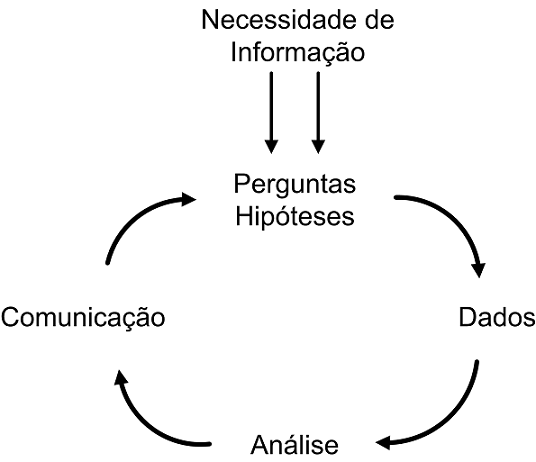
\includegraphics[scale=0.2]{figuras/figura_1} % altere o atributo scale para o tamanho da figura
	\end{center}
	\legend{Fonte: \citeonline{portal_action}}
\end{figure}

\section{PROCEDIMENTOS METODOLÓGICOS}

Procedimentos Metodológicos relaciona-se ao passo-a-passo da execução do trabalho pesquisa: como se obterá os dados necessários para respondem à sua questão de pesquisa? Um bom ponto de partida para escrever os procedimentos é detalhar extensamente cada objetivo específico.

Para que os resultados encontrados sejam considerados válidos, é preciso respeitar e seguir as tradições de cada área de pesquisa. As estratégias de levantamento de dados, e de registro e análise do material coletado, mudam conforme a natureza da pesquisa. Seguem alguns exemplos:


\begin{alineascomponto}
    \item Experimentos, o que inclui desenvolvimento de protótipos ou produtos;
    \item Análise de documentos;
    \item Entrevistas, em duas diversas variações;
    \item Observações, em suas diversas variações;
    \item Metodologia de desenvolvimento de software considerada;
    \item Características das ferramentas a serem utilizadas, e demais recursos necessários;
    \item Para cada uma das estratégias exemplificadas, deve-se responder: 
    \item O que? (atividade)
    \item Como? (técnica)
    \item Quando? (período), podendo ser apresentado apenas no cronograma.
    \item Campo da pesquisa e a amostra de dados a ser considerada (quando aplicável)

\end{alineascomponto}

Quando se tratar de desenvolvimento de ferramenta, vários dos itens anteriormente sugeridos serão substituídos pelo método de desenvolvimento utilizado.

\subsection{Subseção 1}

Se necessário, detalha-se as etapas em subseções. Na primeira versão do projeto, sugere-se usar generosa quantidade de subseções, mesmo que elas fiquem com pouco conteúdo no início. Em versões mais amadurecidas, pode-se unir subseções em grupos, desde que a apresentação do conteúdo de cada uma delas já esteja saturada.
O primeiro passo dos procedimentos não deve ser “revisão bibliográfica” ou “estudar tal e tal conceito”. Conforme \citeonline{wazlawick2014metodologia}, estudar é obrigação do pesquisador, e não uma etapa da pesquisa.

Aceita-se revisão bibliográfica como primeiro passo apenas em casos muito específicos, em uma área do conhecimento muito nova, e que ainda não se tem o conhecimento já desenvolvido e publicado. 

\subsection{Subseção 2}

Ao escrever o passo sobre “análise” ou “avaliação”, é imprescindível informar quais os critérios de análise. Tais critérios, já estarão detalhados na seção de fundamentação teórica, e serão apenas citados nesta seção de procedimentos metodológicos.

\subsection{Cronograma de Execução}

\textit{A última seção dos procedimentos é o cronograma. Apresente a versão que entregará à banca ao final do semestre. Se seus procedimentos não estiverem organizados em subseções, esta será a subseção 4.1. Após ler, remova este texto explicativo.}

\begin{table}[H]
\centering
\resizebox{\textwidth}{!}{\begin{tabular}{|l|c|c|c|c|c|c|c|c|c|c|c|c|c|c|}
\hline
\multicolumn{1}{|c|}{\multirow{2}{*}{ATIVIDADES}} & \multicolumn{14}{c|}{2015} \\ \cline{2-15} 
\multicolumn{1}{|c|}{} & \multicolumn{2}{c|}{Mai} & \multicolumn{2}{c|}{Jun} & \multicolumn{2}{c|}{Jul} & \multicolumn{2}{c|}{Ago} & \multicolumn{2}{c|}{Set} & \multicolumn{2}{c|}{Out} & \multicolumn{2}{c|}{Nov} \\ \hline
\begin{tabular}[c]{@{}l@{}}(escreva aqui a primeira etapa DA EXECUÇÃO,\\  prevista para antes do término do TCC1)\end{tabular} & x & x & x &  &  &  &  &  &  &  &  &  &  & - \\ \hline
Defesa do projeto &  &  &  & x &  &  &  &  &  &  &  &  &  & - \\ \hline
(descreva aqui a segunda etapa da execução) &  &  &  &  & x & x &  &  &  &  &  &  &  & - \\ \hline
(descreva aqui a terceira etapa da execução) &  &  &  &  &  & x & x &  &  &  &  &  &  & - \\ \hline
(descreva aqui a quarta etapa da execução) &  &  &  &  &  &  & x & x &  &  &  &  &  & - \\ \hline
......inclua mais linhas se necessário &  &  &  &  &  &  &  & x &  &  &  &  &  & - \\ \hline
(Execução/coleta de dados de ...) &  &  &  &  &  &  &  & x & x & x &  &  &  & - \\ \hline
(Análise dos Dados) &  &  &  &  &  &  &  &  &  & x & x &  &  & - \\ \hline
(Avaliação da Execução) &  &  &  &  &  &  &  &  &  &  & x & x &  & - \\ \hline
Revisão final da monografia &  &  &  &  &  &  &  &  &  &  &  & x & x & - \\ \hline
Defesa do Trabalho Final &  &  &  &  &  &  &  &  &  &  &  &  & x & - \\ \hline
\end{tabular}}
\end{table}

\section{RESULTADOS PRELIMINARES}

Esta seção estará em vazia na primeira versão de projeto a ser entregue na disciplina Projeto de Pesquisa. Deve ficar vazia mesmo, não sendo excluída.

Após esta entrega, está previsto que a pesquisa seja iniciada e este é o local reservado para que se incluam resultados parciais antes da defesa. Para a defesa, deve-se combinar previamente com o orientador se haverá material suficiente que justifique manter esta seção. Em caso positivo, ela conterá o relato do andamento do trabalho a ser apresentado para a banca avaliadora. Em caso negativo, esta seção é excluída.

% ----------------------------------------------------------
% ELEMENTOS PÓS-TEXTUAIS
% ----------------------------------------------------------
%\postextual

% Referências bibliográficas

\renewcommand{\refname}{REFERÊNCIAS}
\bibliography{bibtex/referencias}
\addcontentsline{toc}{section}{REFERÊNCIAS}
      
% Glossário (Consulte o manual da classe abntex2 para orientações sobre o glossário)
%\glossary

% Apêndices
\apendice{APÊNDICE A}
\addcontentsline{toc}{section}{APÊNDICE A}

Contém materiais de leitura opcional e complementar produzidos pelo autor da pesquisa, incluindo os instrumentos de coleta de dados a serem utilizados. Se não for utilizada, esta seção deve ser removida já na versão 1 do projeto.

% Anexos
% ----------------------------------------------------------
% Anexos
% ---
% Inicia os anexos
% ---

\apendice{ANEXO A}
\addcontentsline{toc}{section}{ANEXO A}

Contém documentos de outros autores, quando aplicável. Se não for utilizada, esta seção deve ser removida já na versão 1 do projeto.

%---------------------------------------------------------------------
% INDICE REMISSIVO
%---------------------------------------------------------------------
%\phantompart
%\printindex
%---------------------------------------------------------------------

\end{document}